%\subsection{Background and Motivation}
% the importance of disaster response -> robots replace humans 
Natural and human-made disasters pose immediate threats to life and infrastructure, requiring rapid and coordinated emergency response. In hazardous environments such as indoor fires, high temperature, dense smoke, and structural instability make human intervention extremely dangerous. 
% Whether to put some case studies such as 香港大浦火灾
% As a result, mobile robots have become a promising alternative for operating in life-threatening spaces, providing fast situational awareness, autonomous exploration, and target search capabilities without exposing emergency responders to unnecessary risk.
A recent devastating fire in Tai Po, Hong Kong~\cite{Grundy2025TaiPoFire} greatly impeded human access and situational awareness during the early response phase, leading to significant casualties and property damage. It was the deadliest fire in Hong Kong in decades.

Mobile robots have emerged as a promising alternative for operating in life-threatening environments. By enabling autonomous exploration, hazard perception, and target search under severe perception degradation, robotic systems can provide rapid situational awareness while reducing the risk to human responders and supporting more informed decision-making.

% single robot exploration
Despite recent progress, most existing search and rescue (SAR) deployments~\cite{queralta2008collaborative} still rely on \emph{single-robot exploration} or loosely coordinated multi-robot routines, where individual robots operate with minimal information sharing. Such strategies inherently limit system-level efficiency, particularly in large, unmapped, or dynamically evolving indoor environments, thereby underscoring the urgent need for multi-agent cooperative navigation. 
%To better illustrate the benefits and challenges of multi-agent search and rescue in such hazardous settings, 
Fig.~\ref{fig:scenario} shows an example scenario of multi-agent search and rescue in an indoor fire environment.
% Given that every second is critical in disaster response, these limitations underscore the urgent need for hazard-aware multi-agent collaborative navigation that can reduce exploration latency and improve overall search effectiveness.
% In these settings, inefficient coverage of vast unknown areas, susceptibility to single-robot failures, and delays caused by incorrect decisions or unexpected obstacles can cumulatively degrade mission performance. 
\begin{figure}
    \centering
    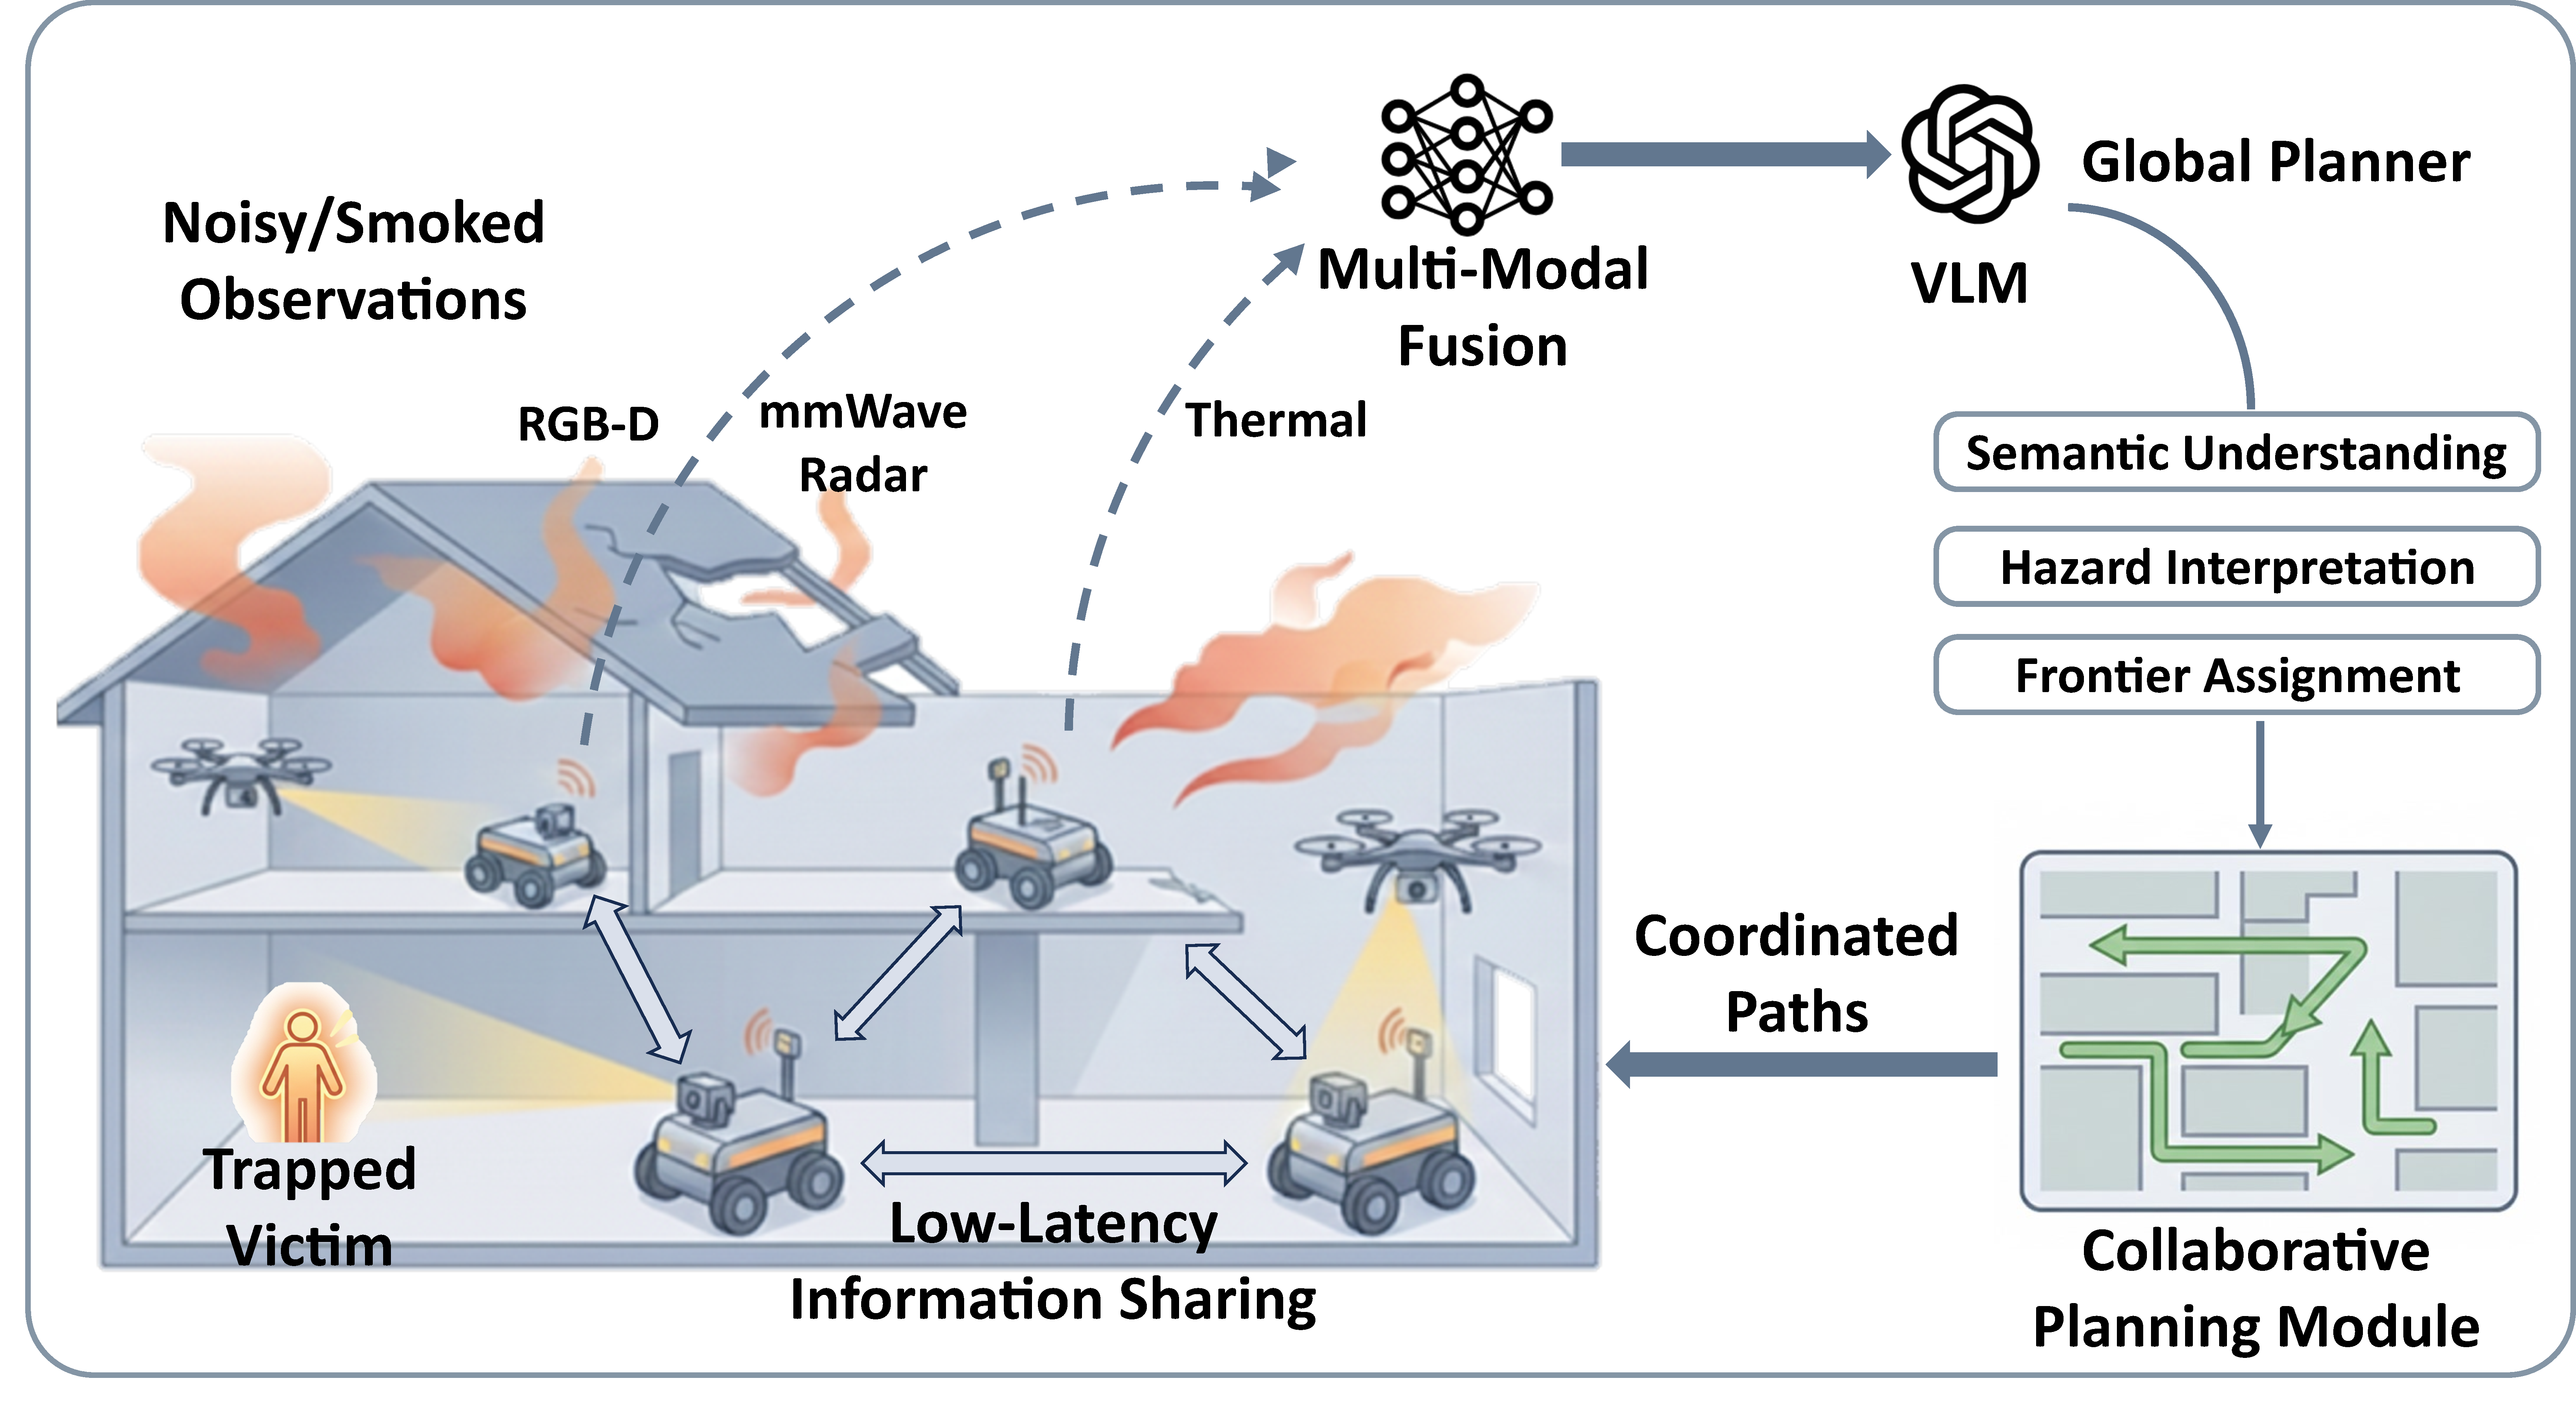
\includegraphics[width=1.0\linewidth]{figures/scenario.pdf}
    \caption{Overview of \system for multi-agent search and rescue in indoor fire scenarios.}%, illustrating sensor observations, multi-modal fusion, VLM-based planning, and coordinated navigation. }
    \label{fig:scenario}
    \vspace{-15pt}
\end{figure}
% 引出视觉导航和VLM导航
\begin{figure}[htbp]
    \centering

    \subfloat[RGB camera]{
        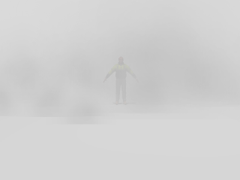
\includegraphics[width=0.45\linewidth]{figures/degradedsensorperformance/rgb.png}
        \label{fig:rgb}
    }
    \hfill
    \subfloat[Depth camera]{
        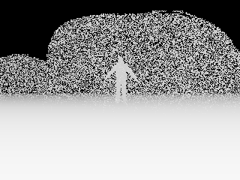
\includegraphics[width=0.45\linewidth]{figures/degradedsensorperformance/depth.png}
        \label{fig:depth}
    }

    %\vspace{0.3cm} % 两行间距，可根据需要调整

    \subfloat[Lidar]{
        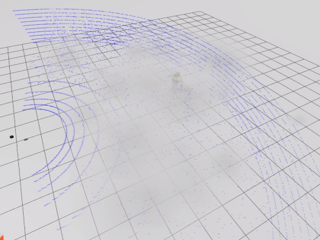
\includegraphics[width=0.45\linewidth]{figures/degradedsensorperformance/lidar.png}
        \label{fig:lidar}
    }
    \hfill
    \subfloat[Thermal camera]{
        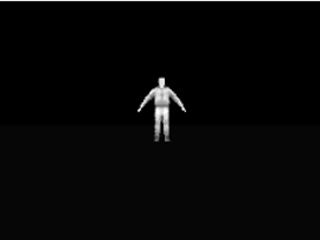
\includegraphics[width=0.45\linewidth]{figures/degradedsensorperformance/thermal.png}
        \label{fig:thermal}
    }

    \caption{Gazebo-based fire simulation demonstrates the degradation of modality-dependent perception  as smoke density increases.}
    \vspace{-15pt}
    \label{fig:four_sensors}
\end{figure}


In recent years, vision-based cooperative navigation has attracted increasing attention, driven by advances in simulation platforms, 
%~\cite{koenig2004design,savva2019habitat}, 
and large-scale 3D scene datasets~\cite{ramakrishnan2021habitat}. Existing approaches to visual navigation are typically grouped into two main paradigms: \emph{end-to-end} systems~\cite{khandelwal2022simple}, which directly map sensory observations to control actions, and \emph{modular pipelines}~\cite{ramakrishnan2022poni}, which explicitly decompose the task into perception, mapping, planning, and control. Both paradigms have demonstrated effectiveness by leveraging spatial and semantic representations learned via supervised or reinforcement learning. Furthermore, recent work has increasingly explored the integration of vision–language
models (VLMs) into visual navigation systems~\cite{11302789}.
%,shen2025enhancing}. 
By jointly reasoning over visual observations and natural language, VLMs introduce powerful semantic priors that enhance object grounding, relational reasoning, and holistic understanding of complex indoor environment. 
%, offering clear performance advantages and emerging as a promising research direction.

However, the majority of existing multi-agent cooperative navigation frameworks~\cite{11302789,liu2024air,yu2022learning} are predominantly vision-based and developed under assumptions of static, well-structured, and relatively benign indoor environments. Such assumptions fundamentally break down in fire-driven indoor scenarios, where perception is severely degraded by smoke and high temperatures, environmental conditions evolve rapidly and unpredictably, and inefficient or uncoordinated exploration can directly compromise both agent safety and mission success. These problems highlight a critical gap in current navigation frameworks and motivate the need for an efficient and safe cooperative multi-agent navigation tailored for indoor fire-disaster response.

\begin{figure*}[t]
  \centering
  \includegraphics[width=\textwidth]{figures/SystemDesign.pdf}
  \caption{System architecture of \system. Each agent performs multi-modal perception and fusion, constructs hazard-aware global maps, and plans safe and efficient exploration using a GNN-based global planner (distilled from a VLM teacher) and a hazard-aware FMM local planner.}
  \label{fig:System Design}
  \vspace{-15pt}
\end{figure*}

%\subsection{Challenges and Contributions}
Despite recent advancements in cooperative navigation including learning-based approaches~\cite{khandelwal2022simple}, VLM powered planning~\cite{11302789}, and embodied multi-agent coordination frameworks~\cite{tan2025roboos}, directly applying these approaches to fire-driven indoor scenarios remains extremely challenging. Compared to static or benign environments, indoor fire scenes introduce several fundamental challenges:

\subsubsection{Dynamic and rapidly evolving environments} 
Temperature gradients, flame propagation, and smoke diffusion continuously reshape the environment, altering traversability, visibility, and semantic cues over time.

\subsubsection{Unreliable and degraded sensor data} 
Fire-induced smoke severely degrades multi-modal perception in indoor environments. 
% Dense smoke scatters and absorbs visible light, significantly impairing RGB-D sensing, while airborne particles directly interfere with LiDAR beams, leading to reduced valid returns as well as spurious measurements such as false echoes and ghost artifacts. In contrast, thermal sensing is comparatively less affected, as it relies on emitted heat rather than optical transparency. 
As illustrated in Fig.~\ref{fig:four_sensors}, our Gazebo-based fire simulations, built on a high-fidelity physics engine with particle-emitter support, qualitatively demonstrate modality-dependent perception degradation under increasing smoke density. 
%, highlighting the fundamental challenges of reliable perception and mapping in fire scenarios.

\subsubsection{Latency-critical and hazard aware decision making} 
SAR missions demand real-time coordination, as excessive planning delays or inefficient multi-robot routing can directly compromise human survival and overall mission success. Simultaneously, it is crucial to ensure that each agent can navigate and explore safely, avoiding hazards while completing its tasks. Recent VLM-based global planners~\cite{11302789} provide strong common-sense priors for frontier assignment, but each call blocks for ${\sim}20$\,seconds of network round-trip and remote inference, incurs a per-call API cost, requires reliable connectivity, and is non-deterministic across runs. In a fire scene this is unacceptable: a 5-minute safe operating window can be entirely consumed by API wait time, the network link itself may degrade with smoke or radio interference, and on-board fall-back behavior is needed when the cloud is unreachable. \emph{This motivates replacing the VLM in the global-planner loop with a small, on-board model that preserves the VLM's coordination quality while reducing per-decision latency by orders of magnitude.}

% To address these challenges, we introduce \textbf{\system}\footnote{\system is the Roman deity of fire.}, a novel hazard-aware multi-agent cooperative navigation framework tailored for indoor fire scenarios. 
% % Introduce the system breifly
% The implementation and evaluation of our \system will be a future work.
% We provide a project website \href{https://vulcan-dr.github.io}{https://vulcan-dr.github.io}, which showcases live demonstrations as well as representative preliminary results. 
To address these challenges, we introduce \textbf{\system}\footnote{\system is the Roman deity of fire.}, a hazard-aware multi-agent cooperative navigation framework tailored for indoor fire SAR scenarios. As illustrated in Fig. ~\ref{fig:scenario}, each agent performs multi-modal perception and fusion to jointly construct a hazard-aware global map. Based on this shared representation, exploration is coordinated through a \emph{graph neural network (GNN) global planner}---distilled from a GPT-4o teacher via behavior cloning---and a hazard-aware local planner to ensure safe and efficient navigation. The GNN operates on a bipartite robot--frontier graph, contains fewer than $10^5$ parameters, runs fully on board in ${\sim}3$\,ms per decision, and matches the VLM teacher's success rate on HM3D while being ${\sim}6{,}100\times$ faster. While a complete end-to-end deployment is ongoing, we implement key components and present preliminary evaluations demonstrating the framework’s feasibility and the limitations of conventional multi-agent navigation in fire scenarios. Live demonstrations and representative results are available at \url{https://vulcan-dr.github.io}.


% We provide a project website \href{https://vulcan-dr.github.io}{https://vulcan-dr.github.io}, which presents live demonstrations and representative results.

% While a complete end-to-end deployment is ongoing, we implement key components and present preliminary evaluations demonstrating the framework’s feasibility and the limitations of conventional multi-agent navigation in fire scenarios. A project website (\href{https://vulcan-dr.github.io}{https://vulcan-dr.github.io}
% ) provides live demonstrations and representative results.
To summarize, our contributions are as follows:
\begin{itemize}
    \item We propose \system, a hazard-aware multi-agent cooperative navigation framework tailored for indoor fire scenarios, which maintains high navigation efficiency despite severe fire-induced perception degradation and environmental hazards.
    \item We replace the VLM in the global-planner loop with a lightweight \emph{GNN student} ($<\!10^5$ parameters) that operates on a bipartite robot--frontier graph and is distilled from GPT-4o decisions via behavior cloning, removing the cloud dependency, the per-call API cost, and the ${\sim}20$\,s decision latency that block on-board deployment.
    \item We extend indoor navigation benchmarks with realistic fire simulations and couple the GNN-based global planner with a hazard-aware local controller.
    \item We evaluate representative multi-agent navigation baselines, the GPT-4o teacher, and our GNN student under both normal and simulated indoor fire conditions, and systematically analyze the underlying causes of their performance degradation in fire scenarios.
\end{itemize}



